\chapter{Implementation}
Before being able to develop a second working prototype that implements some of the functionality it is needed a fully functional back-end component. This chapter describes how this was was achieved with the elected design and technological choices going from the development of each back-end component to the development and implementation of a second and a third prototype.
\section{Back-end}

\iffalse
\subsection{Environment setup}
Following the design and technological choices from the previous chapter; the dedicated hardware components were launched from Amazon Web Services. 
\fi

\subsection{Web crawler}
A web crawler is a service that automatically browses the web and extracts useful information to later insert it into a persistent storage. The air quality data needed to feed the application will be extracted from the Air Quality in Scotland website (REF) as discussed in previous chapters. Scrappy was the selected technology for this purpose. The way scrappy extracts structured data from a web-page is by browsing the HTML document with XPATH expressions. 

\begin{figure}[H]
\begin{adjustbox}{width=.5\textwidth,center=\textwidth}
  \centering
  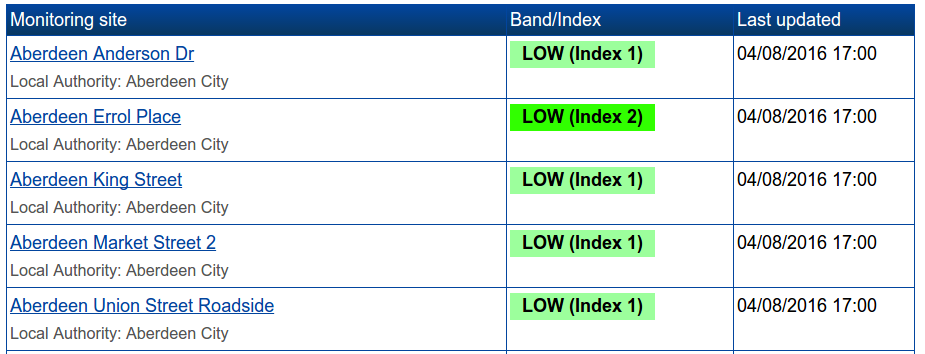
\includegraphics[scale=1]{images/monitoring_summary.png}
\end{adjustbox}
  \caption[Pollution sensors list]{Pollution sensors list \footnotemark}
  \label{fig:pollution_sensors_list}
\end{figure}
\footnotetext{\url{http://www.scottishairquality.co.uk/latest/summary}}

The website data source contains many sensors from different authorities in Scotland as shown in Figure \ref{fig:pollution_sensors_list}, they aggregate the data and display a list of the available sensors. The first thing the crawler would need to do is to extract the links to navigate through all the available sensors. The rendered sensor list table looks like the code bellow in plain HTML. It is noticeable that the XPATH selector needs to go through the table to reach the \textit{href} attribute in order to access the data for that specific sensor. 

To select the \textit{href} attribute: 

{\centering
\begin{BVerbatim}
//tr/td[1]/a@href
\end{BVerbatim}
\par
}

The output of the XPATH selector is highlighted in red: 

\begin{Verbatim}[fontsize=\small,commandchars=\\\(\)]
<table>
  <tbody>
    <tr>
      <td><a href="(\color(red)site-info?site_id=ABD1")>Aberdeen Anderson Dr</a><br></td>
      <td><span>LOW (Index 1)</span></td>
    </tr>
      <tr>
      <td><a href="(\color(red)site-info?site_id=ABD)">Aberdeen Errol Place</a><br></td>
      <td><span>LOW (Index 2)</span></td>
    </tr>
  </tbody>
</table>
\end{Verbatim}

Once that the URL containing the data is extracted, scrappy executes another request to select the interesting data for each sensor. The readings are rendered through a table which contains the pollutant, the band, the concentration and the update period as shown in 

\begin{figure}[H]
\begin{adjustbox}{width=.5\textwidth,center=\textwidth}
  \centering
  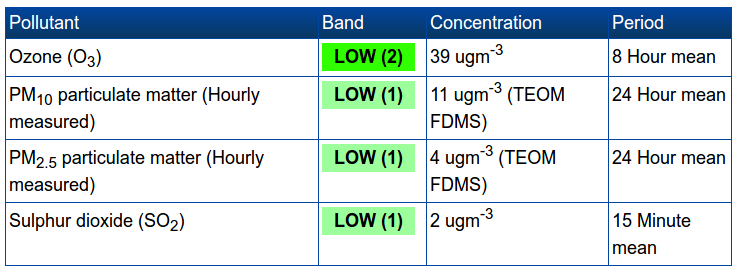
\includegraphics[scale=1]{images/site_readings.png}
\end{adjustbox}
  \caption[Edinburgh St Leonard's site readings]{Edinburgh St Leonard's site readings \footnotemark}
  \label{fig:pollution_site readings}
\end{figure}
\footnotetext{\url{http://www.scottishairquality.co.uk/latest/site-info?site_id=ED3}}


This time, all the information contained in a \textit{td} tag is selected. 

\begin{Verbatim}[fontsize=\small,commandchars=\\\(\)]
<table>
  <tbody>
    <tr>
      <td>Ozone (O<sub>3</sub>)</td>
      <td><span class="band index2">LOW (2)</span></td>
      <td>39 ugm<sup>-3</sup></td>
      <td>8 Hour mean</td>
    </tr>
  <tr>
    <td>PM<sub>10</sub> particulate matter (Hourly measured)</td>
    <td><span class="band index1">LOW (1)</span></td>
    <td>11 ugm<sup>-3</sup> (TEOM FDMS)</td>
    <td>24 Hour mean</td>
  </tbody>
</table>                
\end{Verbatim}



\subsection{Database}
\subsection{Advice service}


\section{Front end implementation}
\subsection{User interface}
\subsection{Visualizations}
\subsection{Demo mode}

\section{Testing}
Tested through the Amazon Mobile Hub

\section{Deployment}
The application was uploaded to the Android Market a